\documentclass[9pt, aspectratio=169]{beamer}
\usepackage{FiraSans}
\usetheme[subsectionpage=progressbar]{metropolis}
\usepackage[utf8]{inputenc}
\usepackage{amsmath}
\usepackage{amsfonts}
\usepackage{amssymb}
\usepackage{multicol}
\usepackage{tikz}
\usepackage{xcolor}
\usepackage[T1]{fontenc} 
\usepackage[skins]{tcolorbox}
\author{Nicola Roman\`o - nicola.romano@ed.ac.uk}
\title{Lecture 1 - Introduction to image analysis}
\setlength{\fboxsep}{0pt}
\setbeamertemplate{caption}{\raggedright\insertcaption\par}
\setbeamertemplate {footline}{\begin{scriptsize}\hfill\insertframenumber ~of \inserttotalframenumber\kern1em\vskip5pt\end{scriptsize}}

%\setbeamercovered{transparent} 
%\setbeamertemplate{navigation symbols}{} 

\titlegraphic{\centering 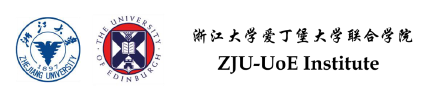
\includegraphics[scale=.5]{instituteLogo.png}}
\date{}

\begin{document}

\newtcolorbox{codebox}{enhanced,
    top=2pt,
    left=2pt,
    right=2pt,
    bottom=2pt,
    boxrule=0pt,
    leftrule=5pt,
    sharp corners,
    colback=gray!20,
    colframe=blue!60!black}

\begin{frame}
    \titlepage
\end{frame}

\section{Introduction to the course}

\begin{frame}
    {Biomedical image analysis 4}

    \begin{columns}
        \begin{column}{0.6\textwidth}
            Semester 1 only course, 20 UoE credits / 5 ZJU credits.\\
            CO : Nicola Roman\`o - nicola.romano@ed.ac.uk\\
            \vspace{2em}
            This course contributes 3.3\% of the final ZJU GPA or 3.6\% of the final GPA for international students.\\
            \vspace{2em}
            This course contributes 11.1\% of the final UoE degree mark used for degree classification.\\
            \vspace{2em}

            \onslide<2>{This course aims to give you the ability to apply and improve strategies and pipelines for biomedical image analysis.}
        \end{column}
        \begin{column}{0.3\textwidth}
            \begin{figure}
                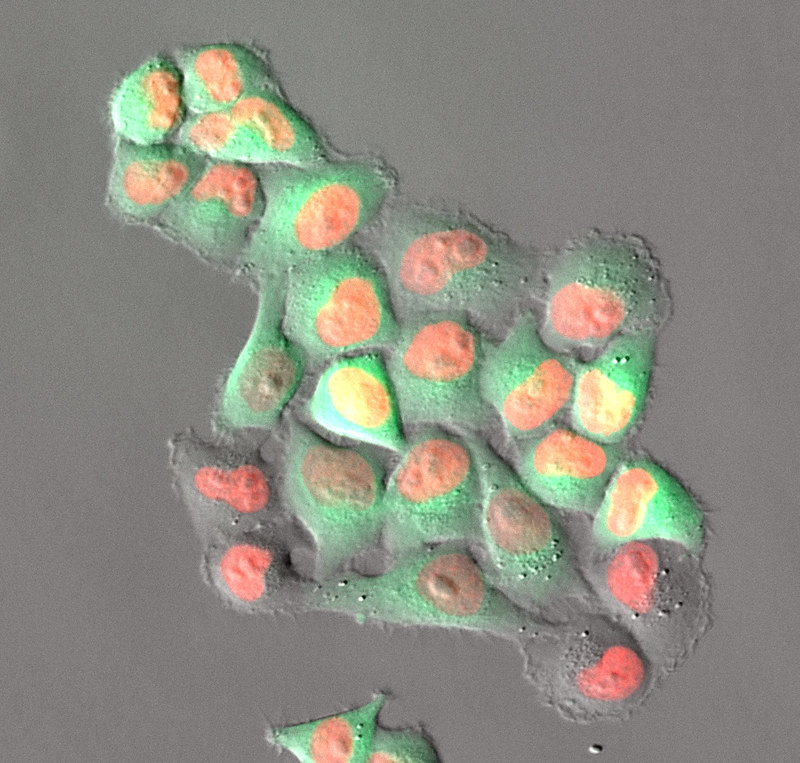
\includegraphics[width=\textwidth]{cells.jpg}
                \caption{\color{gray}{Zeiss - CC-BY-2.0}}
            \end{figure}
        \end{column}
    \end{columns}
\end{frame}

\begin{frame}
    {Learning outcomes}
    \begin{itemize}
        \item Describe and critically discuss strategies and algorithms for analysis of biomedical images
        \item Implement these strategies using Python
        \item Work in a team to critically address a real-life problem involving image analysis by developing and applying an appropriate pipeline
        \item Professionally document their analysis, presenting their pipeline and the results of their analysis, in the context of the biomedical problem it is aiming to solve.
    \end{itemize}
    \vspace{2em}
    Please see the course handbook for more information
\end{frame}

\begin{frame}
    {Assessment}

    \textbf{ICA 1 – Group work – 40\% final mark}

    You will produce a well-documented piece of Python software to solve a specific problem in bio-imaging.

    \textbf{ICA 2 – Individual work – 60\% final mark}

    You will produce an individual report highlighting the use for your software and reflecting on your group work.

    \vspace{2em}
    Specific information on the ICAs will be given later during the course.
\end{frame}

\begin{frame}
    {What will we talk about}
    \begin{columns}
        \begin{column}{0.7\textwidth}
            \begin{itemize}[<+->]
                \item \textit{Lectures 1-5} - Basic operations on images (e.g. displaying, cropping, rotating, \dots), filtering and image enhancement.
                \item \textit{Lectures 6-8} - More complex operations (e.g. feature extraction, tracking, segmentation, \dots).
                \item \textit{Lectures 9-16} - Traditional and modern (deep learning) machine learning methods for image analysis
                \item \textit{Lectures 17-20} - Discussion on recent topics in image analysis
            \end{itemize}
        \end{column}

        \begin{column}{0.3\textwidth}
            \begin{figure}
                
\includegraphics[width=\textwidth]{notes.jpg}
                \caption{\color{gray}{Matt Cornock - CC BY-NC 2.0}}
            \end{figure}
        \end{column}
    \end{columns}
    A complete timetable is available on Learn.
\end{frame}

\begin{frame}
    {Use of Python in the course}
    We will cover both the theory and practical aspects (with Python code!) of these topics.\\

    You will have \textbf{Python workshops} to practice these problems first hand.\\

    \pause

    Please note that \textbf{you will need Python knowledge} to pass this course. You can find \textbf{introductory material} on Learn, to learn the basics of Python or refresh your knowledge.

    \pause

    I will also post \textbf{quizzes} on Learn after most lectures, to reinforce your understanding and \textbf{extra reading material} that will be useful to expand your image analysis knowledge.\\
\end{frame}

\begin{frame}
{Attendance}
Please note that attendance is \textbf{mandatory} for this course.\\
Attendance will be recorded in all sessions (but for today).\\
Students who miss more than 10\% of the sessions might force-fail the course.\\

Please see the Course and the Programme handbooks for more information.
\end{frame}

\begin{frame}
    {Asking for help}
    \begin{center}
        
\includegraphics[width=0.1\textwidth]{slack.png}
    \end{center}

    You have been added to a \textbf{Slack} group. Please join and introduce yourself, if you have not already!

    This is an invaluable opportunity to discuss anything related to the course (including your ICA!) with your peers and the course staff.    

    Introductory material about Python is available on Learn and further material can be provided, if needed - plase ask!    
\end{frame}

\begin{frame}
    \section {Introduction to image analysis}
\end{frame}

\begin{frame}
    {Learning objectives}
    \begin{columns}
        \begin{column}{0.8\textwidth}
            \begin{itemize}
                \item Give examples of problems in image analysis
                \item Describe common Python libraries used in image analysis
                \item Describe images as matrices or tensors
                \item Display images using Python
            \end{itemize}
        \end{column}
        \begin{column}{0.2\textwidth}
            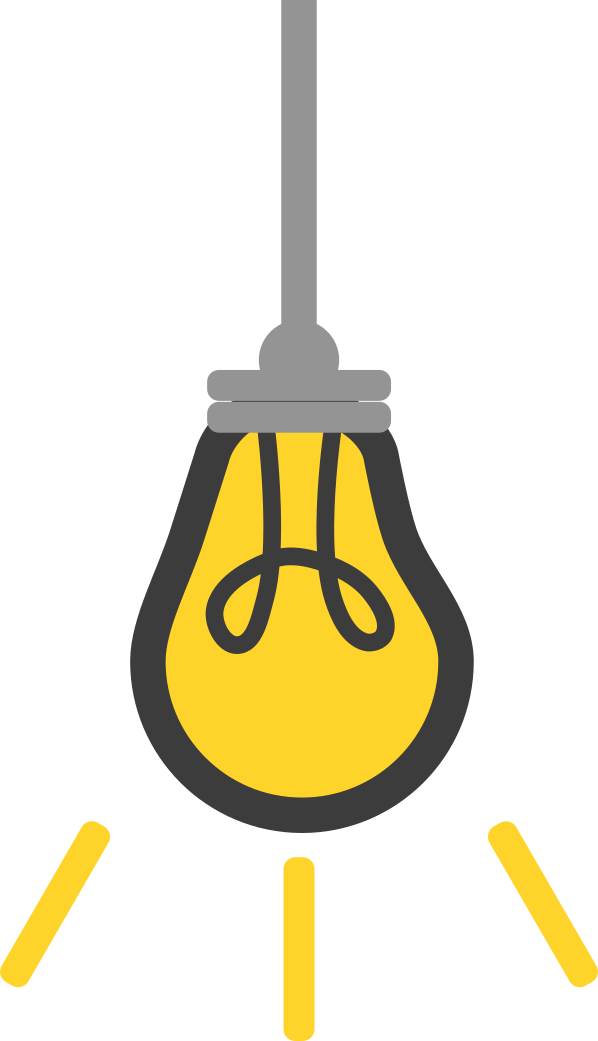
\includegraphics[angle=-30, origin=tr, width=1.5\textwidth]{lightbulb.png}
        \end{column}
    \end{columns}
\end{frame}

\section{Why do we need to analyse images?}

\begin{frame}
    {Examples of biomedical images and associated problems}
    Image processing is a major task in biomedical sciences (and not only).
    Problems in image analysis include detection of objects; quantification of their properties; improvement of image quality; classification of images\dots

    \begin{columns}
        \begin{column}{0.25\textwidth}
            \begin{figure}
                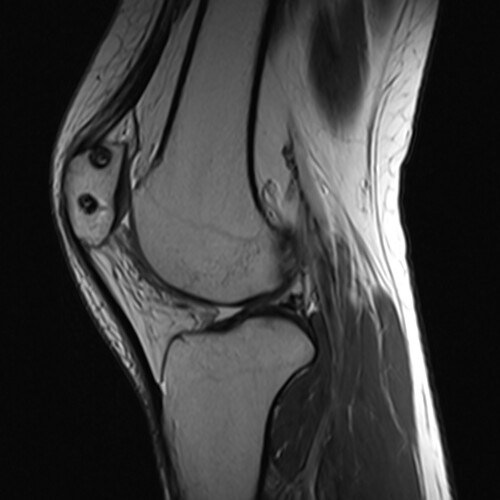
\includegraphics[height=10em]{MRI - Becky Stern CC-BY-SA2.jpg}
                \caption{\color{gray}{Becky Stern - CC-BY-SA 2.0}}
            \end{figure}
        \end{column}
        \begin{column}{0.25\textwidth}
            \begin{figure}
                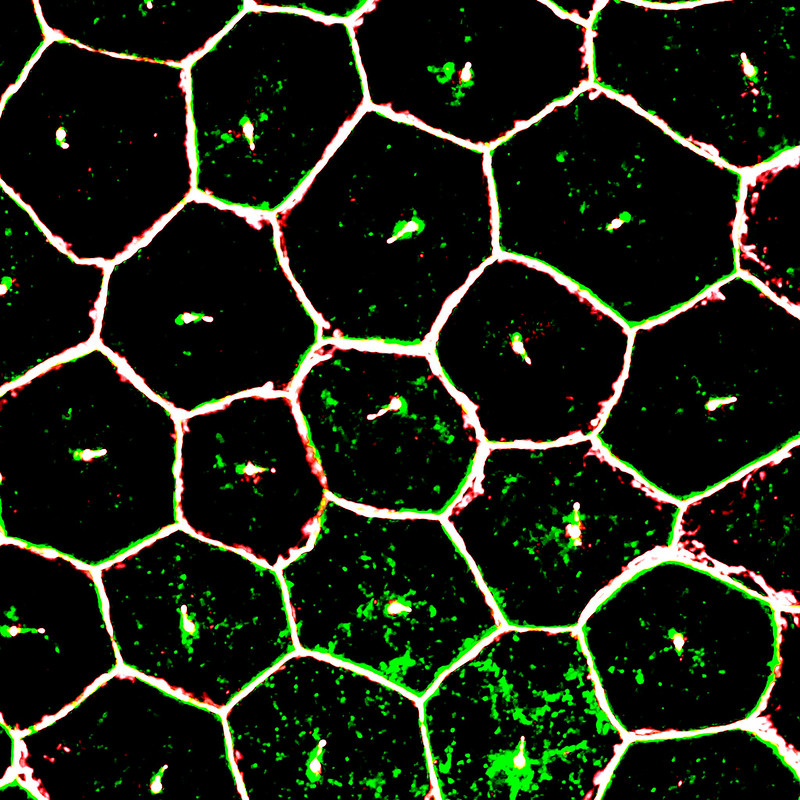
\includegraphics[height=10em]{Retinal pigment epithelium - NIH - CC BY-NC 2.0.jpg}
                \caption{\color{gray}{NIH - CC-BY-SA 2.0}}
            \end{figure}
        \end{column}
        \begin{column}{0.25\textwidth}
            \begin{figure}
                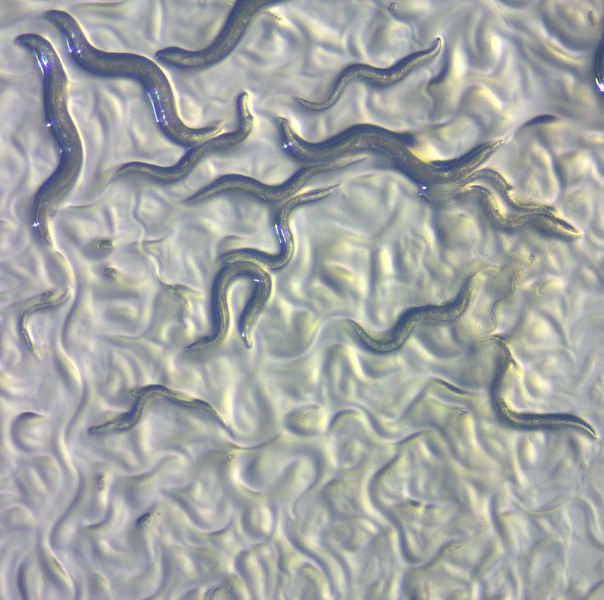
\includegraphics[height=10em]{c elegans - Zeiss - CC-BY 2.0.jpg}
                \caption{\color{gray}{Zeiss - CC-BY 2.0}}
            \end{figure}
        \end{column}
        \begin{column}{0.25\textwidth}
            \begin{figure}
                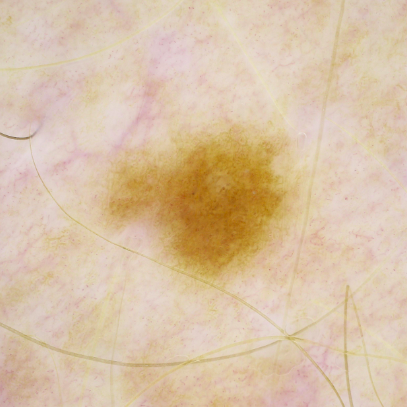
\includegraphics[height=10em]{ISIC melanoma competition - CC0.png}
                \caption{\color{gray}{ISIC melanoma competition - CC-0}}
            \end{figure}
        \end{column}
    \end{columns}

\end{frame}

\begin{frame}
    {Examples of image analysis problems}
    \only<1>
    {
        \begin{figure}
            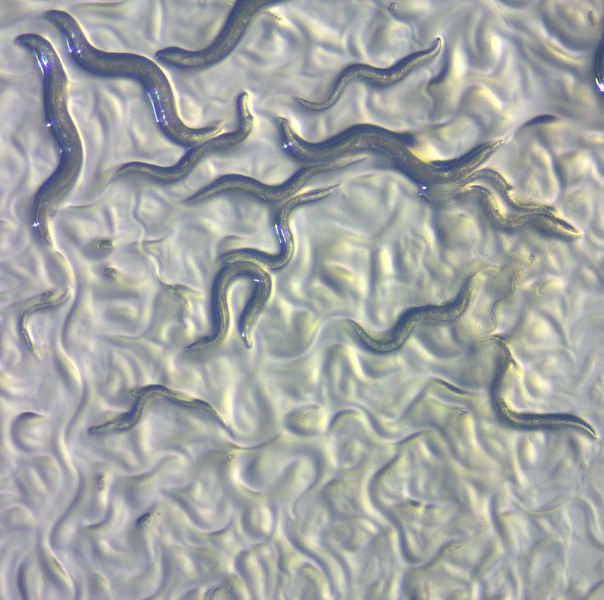
\includegraphics[height=12em]{c elegans - Zeiss - CC-BY 2.0.jpg}
            \caption{\color{gray}{Zeiss - CC-BY 2.0}}
        \end{figure}
        \centering
        How many worms are in this image?\\
        Where are they located?\\
        Where are they moving to (assuming you have a video!)?
    }
    \only<2>
    {
        \begin{figure}
            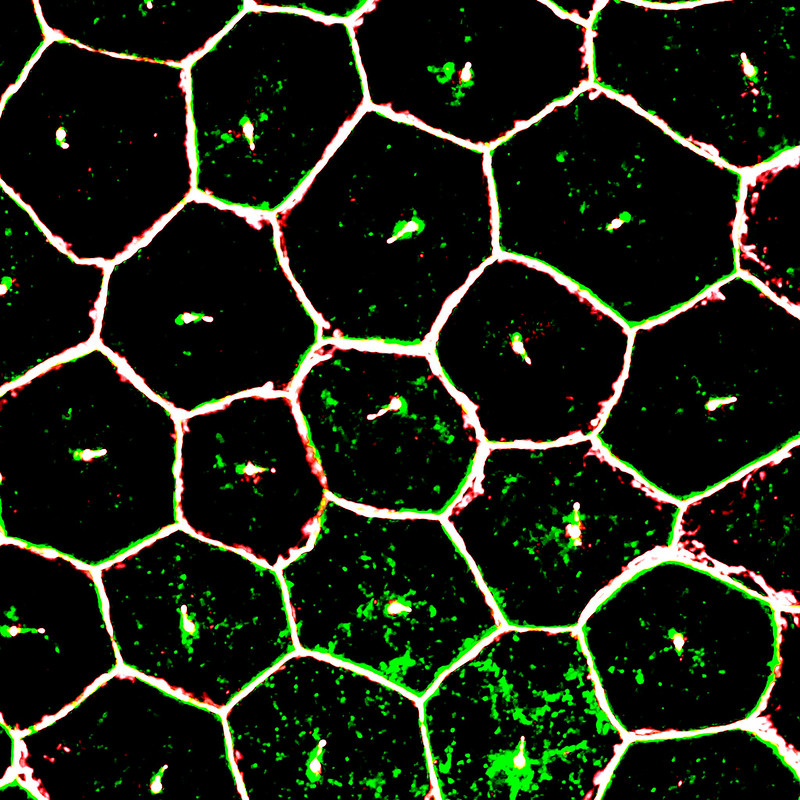
\includegraphics[height=12em]{Retinal pigment epithelium - NIH - CC BY-NC 2.0.jpg}
            \caption{\color{gray}{NIH - CC-BY-SA 2.0}}
        \end{figure}
        \centering
        Where are the cells located?\\
        How intense is the green staining in each cell?\\
        How uniformly is the staining distributed?
    }
    \only<3>
    {
        \begin{figure}
            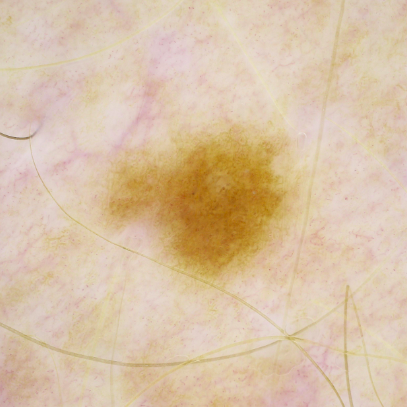
\includegraphics[height=10em]{ISIC melanoma competition - CC0.png}
            \caption{\color{gray}{ISIC melanoma competition - CC-0}}
        \end{figure}
        \centering
        Is this a melanoma?
    }
\end{frame}

\begin{frame}
    {In this course...}
    \centering
    \Large
    We will learn strategies to analyse images and answer this types of questions.

    Let's start with something simple!

\end{frame}

\section{Simple operations with images}

\begin{frame}
{Images as rasters}
When analysing digital images we are concerned with \textbf{rasters}.\\
A raster is a series of \textbf{pixels} arranged in a rectangular grid, which represent an image. Each pixel is associated with a value or a series of values, representing its intensity and colour.
\begin{center}
    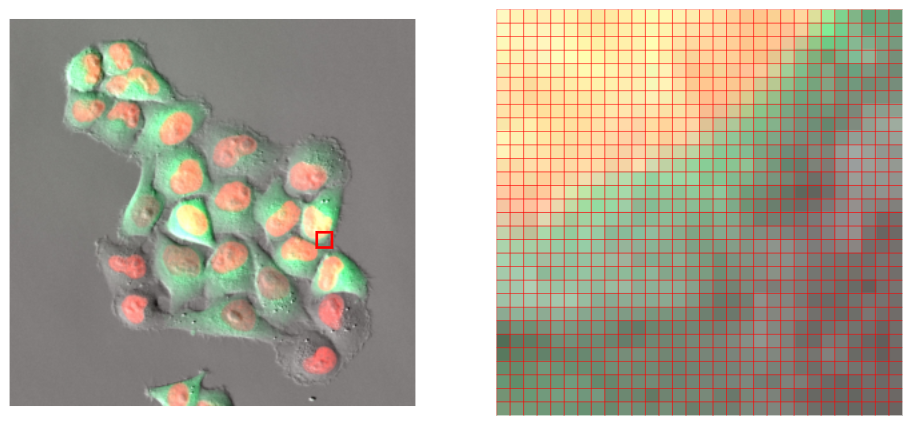
\includegraphics[width=.8\textwidth]{raster.png}
\end{center}
\end {frame}

\begin{frame}
    {Images as matrices (or tensors)}
    Because images are grids of values, we can represent them as matrices.\\

    The dimensions of the matrix will be (width, height).
    For example, if 0 is black and 255 is white (more on this later)

    \begin{columns}
        \begin{column}{0.5\textwidth}
            $$
                \begin{bmatrix}
                    237 & 80  & 46  & 52  & 144 & 151 \\
                    245 & 166 & 190 & 166 & 190 & 245 \\
                    2   & 27  & 76  & 167 & 206 & 222 \\
                    245 & 184 & 163 & 182 & 119 & 83  \\
                    112 & 186 & 253 & 172 & 201 & 43  \\
                    6   & 204 & 230 & 6   & 125 & 134 \\
                \end{bmatrix}
            $$
        \end{column}

        \begin{column}{0.45\textwidth}
            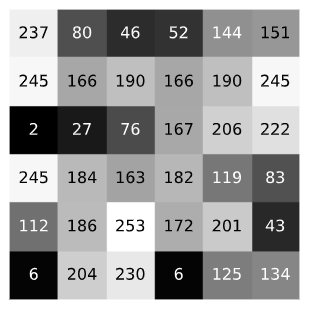
\includegraphics[width=.8\textwidth]{rasterexample.png}
        \end{column}
    \end{columns}
\end{frame}

\begin{frame}
    {What about colour?}
    Colour images are generally stored as RGB (red, green, blue).\\
    The color of each pixel depends on its intensity in each of these three \textbf{colour channels}.

    
\begin{tikzpicture}
        \definecolor{tempcolor}{RGB}{80,0,0}
        \draw [fill=tempcolor](0, 0) rectangle (1, 1);
        \node [align=center,color=white] at (0.5, 0.5) {80};
        \definecolor{tempcolor}{RGB}{0,120,0}
        \draw [fill=tempcolor](1.5, 0) rectangle (2.5, 1);
        \node [align=center,color=white] at (2, 0.5) {120};
        \definecolor{tempcolor}{RGB}{0,0,150}
        \draw [fill=tempcolor](3, 0) rectangle (4, 1);
        \node [align=center,color=white] at (3.5, 0.5) {150};
        \definecolor{tempcolor}{RGB}{80,120,150}
        \draw [-stealth,color=black] (4.5, 0.5) -- (5, 0.5);
        \draw [fill=tempcolor](5.5, 0) rectangle (6.5, 1);
    \end{tikzpicture}
    \pause

    \begin{columns}
        \begin{column}{0.6\textwidth}
            \begin{figure}
                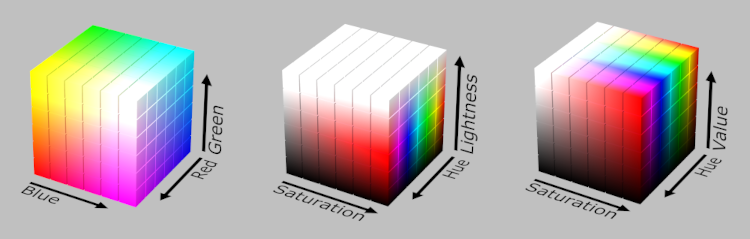
\includegraphics[width=\textwidth]{colorspaces.png}
                \caption{\color{gray}Adapted from Wikipedia}
            \end{figure}
        \end{column}
        \begin{column}{0.4\textwidth}
            RGB is not the only way to represent colour. If you are interested in knowing more about \textbf{colour spaces} see the attached review by Hastings and Rubins, 2012.
        \end{column}
    \end{columns}
    \pause
    Important: microscope images are often composed of multiple grayscale images, e.g. of different fluorophores. In this case, each pixel has multiple colour channels.
\end{frame}

\begin{frame}
    {Storing colour images}
    \begin{columns}
        \begin{column}{.3\textwidth}
            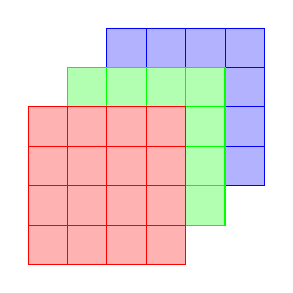
\begin{tikzpicture}
                \draw[step=0.5cm,blue,very thin, fill=white!70!blue] (-2, -2) grid (0, 0) rectangle (-2, -2);
                \draw[step=0.5cm,green,very thin, fill=white!70!green] (-2.5, -2.5) grid (-0.5, -0.5) rectangle (-2.5, -2.5);
                \draw[step=0.5cm,red,very thin, fill=white!70!red] (-3, -3) grid (-1, -1) rectangle (-3, -3);
            \end{tikzpicture}
        \end{column}
        \begin{column}{0.7\textwidth}
            Colour images are stored as a 3-dimensional matrix, also called a \textbf{tensor} with dimensions (number of colour channels, width, height).
        \end{column}
    \end{columns}
    \vspace{2em}
    \pause
    \begin{columns}
        \begin{column}{0.3\textwidth}
            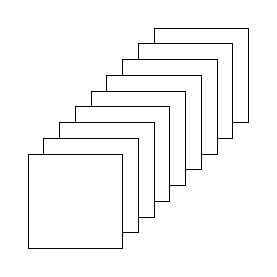
\begin{tikzpicture}
                \foreach \i in {-1,-0.8,...,0.6}
                    {
                        \draw[black,very thin, fill=white] ({-\i+1.2}, {-\i+1.2}) rectangle ({-\i}, {-\i});
                    }
            \end{tikzpicture}
        \end{column}
        \begin{column}{0.7\textwidth}
            Multi-dimensional matrices can be used to represent videos (number of frames, width, height) or stacks of images, e.g. in confocal images, with dimensions (number of planes, width, height).
        \end{column}
    \end{columns}

    \vspace{1em}
    Note that the order of the dimensions might vary.
\end{frame}

\begin{frame}
    {Bit depth}
    \begin{figure}
        \textbf{Bit depth} is the number of bits necessary to represent each pixel in the image.
        \centering
        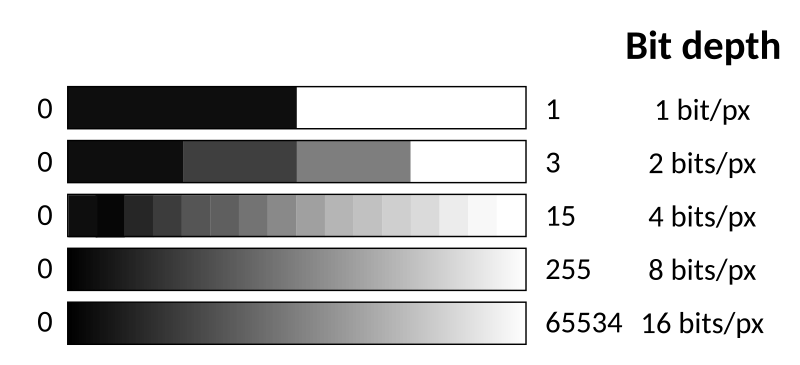
\includegraphics[width=.6\textwidth]{bitdepth.png}
        \caption{Increasing bit depth > Increasing information}
    \end{figure}
    \pause

    You can also represent images with floating-point numbers. In that case, you have infinite levels between [0.0, 1.0] or [-1.0, 1.0].\\
\end{frame}

\begin{frame}
    {Bit-depth app}
    This simple app will show you the effect of changing the bit depth of an image.

    \centering
    
\includegraphics[width=.4\textwidth]{qrcode_bitdepth.png}
\end{frame}

\begin{frame}
    {Representing matrices in Python}
    
\includegraphics[width = 0.3\textwidth]{numpylogo.png}
    The Numpy library simplifies working with matrices in Python.

    NumPy is a Python open-source library for numerical computing, with support for n-dimensional arrays and many functionalities to work with matrices.

    Numpy can be installed via \texttt{pip} in a terminal or command prompt.

    \begin{codebox}
        \texttt{pip install numpy}
    \end{codebox}
\end{frame}

\begin{frame}
    {Our first NumPy matrix!}

    \begin{codebox}
        \texttt{\# This is the standard way of importing numpy\\
            import numpy as np\\
            a = np.array([1, 2, 3])
        }
    \end{codebox}

    \begin{figure}
        \centering
        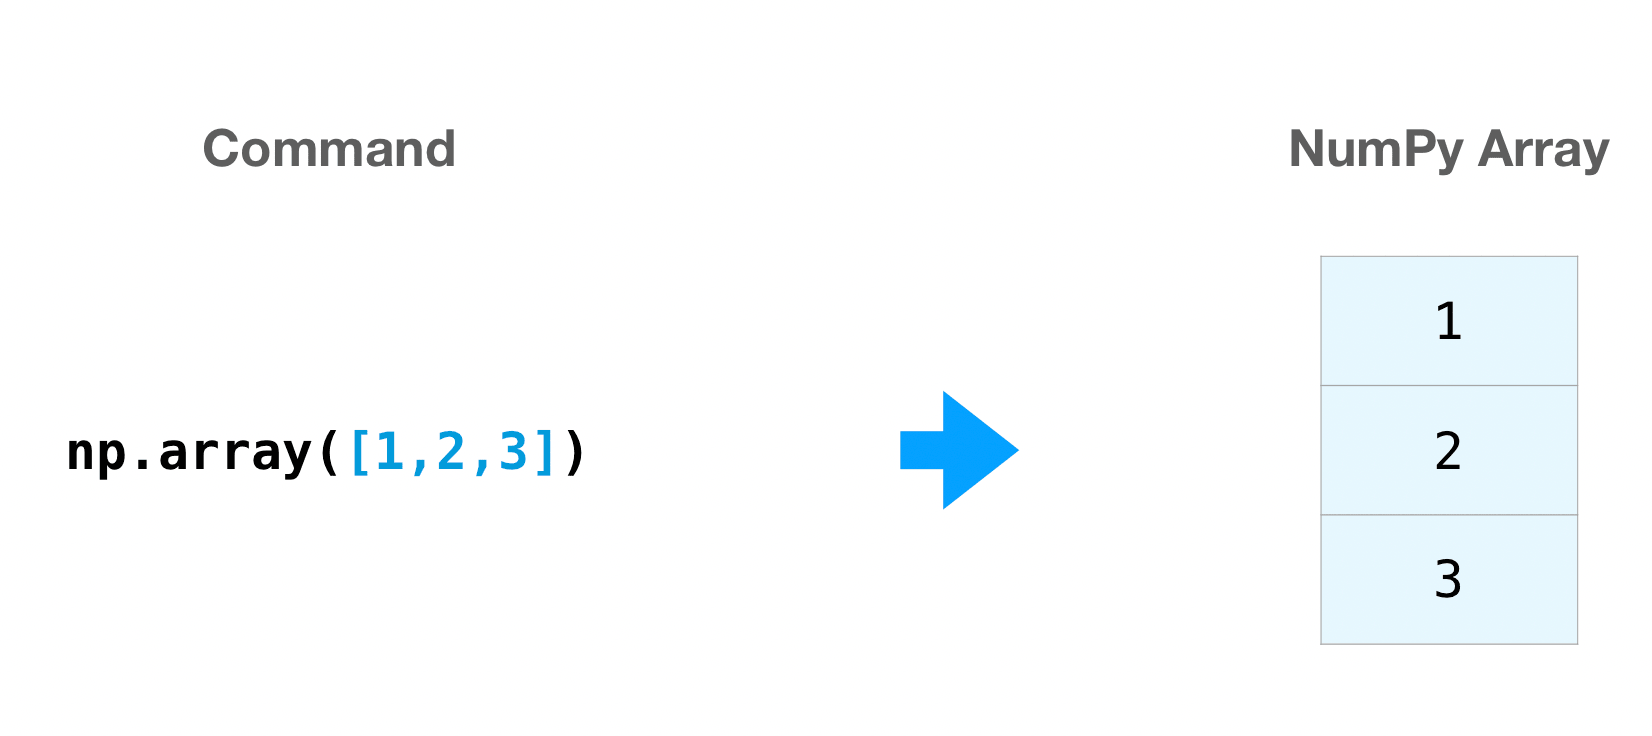
\includegraphics[height=100px]{np_array.png}
    \end{figure}
\end{frame}

\begin{frame}
    {Multiple dimensions}

    Numpy supports n-dimensional arrays with any number of dimensions.

    \begin{codebox}
        \texttt{import numpy as np\\
            b = np.array([[1, 2, 3][4, 5, 6]])\\
            print(b.shape)
        }
    \end{codebox}

    \begin{codebox}
        {
            \texttt{(2, 3)}
        }
    \end{codebox}

    The shape of an array is a vector showing the number of element in each of the dimensions of the array. In this case, we have a matrix of 2 rows by 3 columns.
\end{frame}


\begin{frame}
    {Matrix operations in Python}

    The Numpy library allows easy manipulation of matrices (and thus images).

    \begin{codebox}
        \texttt{import numpy as np\\
            \# We can define a matrix\\
            a = np.array([[10, 15, 20],
                    [20, 25, 30],
                    [120, 5, 20]])\\
            \# Perform basic operations on it\\
            b = a + 10\\
            c = a * 2
        }
    \end{codebox}
    \pause
    $$
        a =
        \begin{bmatrix}
            10  & 15 & 20 \\
            20  & 25 & 30 \\
            120 & 5  & 20 \\
        \end{bmatrix}
        \quad b =
        \begin{bmatrix}
            20  & 25 & 30 \\
            30  & 35 & 40 \\
            130 & 15 & 30 \\
        \end{bmatrix}
        \quad c =
        \begin{bmatrix}
            20  & 30 & 40 \\
            40  & 50 & 60 \\
            240 & 10 & 40 \\
        \end{bmatrix}
    $$
\end{frame}

\begin{frame}
    {More info on Numpy}
    For more information on Numpy

    \begin{columns}
        \begin{column}{.7\textwidth}
            \begin{enumerate}
                \item Check their website \dots
                \item \dots in particular \url{https://numpy.org/devdocs/user/absolute_beginners.html} 
\includegraphics[width=.25\textwidth]{QRnumpy.png}
                \item Check the Numpy paper (Harris et al, Nature 2020, on Learn)
            \end{enumerate}
        \end{column}
        \begin{column}{.3\textwidth}
            
\includegraphics[width=\textwidth, trim=0  0  390  0, clip]{numpylogo.png}
        \end{column}
    \end{columns}
\end{frame}

\begin{frame}
    {Matplotlib and Scikit Image}

    Two very useful libraries to draw and manipulate images are Matplotlib and Scikit Image.
    \begin{center}
        
\includegraphics[width=0.3\textwidth]{matplotlib_logo.png}
        
\includegraphics[width=0.3\textwidth]{skimage_logo.png}
    \end{center}

    Install using
    \begin{codebox}
        \texttt{pip install matplotlib}\\
        \texttt{pip install scikit-image}
    \end{codebox}
    \pause
    \textbf{Matplotlib} - very powerful, general-purpose plotting library. You will generally using by importing the pyplot submodule.\\
    \begin{codebox}
        \texttt{import matplotlib.pyplot as plt}
    \end{codebox}
    \pause
    \textbf{Scikit Image} - built on top of Matplotlib and is specialized for image manipulation and analysis. Contains many submodules to perform specific operations.\\
\end{frame}

\begin{frame}
    {Loading images - Matplotlib vs Scikit Image}

    \begin{columns}
        \begin{column}{0.5\textwidth}
            \begin{center}
                
\includegraphics[width=0.5\textwidth]{matplotlib_logo.png}
            \end{center}
            \begin{codebox}
                \texttt{import matplotlib.pyplot as plt\\
                    img = plt.imread("cells.jpg")\\
                    plt.imshow(img)\\
                    plt.show()
                }
            \end{codebox}
        \end{column}
        \pause
        \begin{column}{0.5\textwidth}
            \begin{center}
                
\includegraphics[width=0.5\textwidth]{skimage_logo.png}
            \end{center}
            \begin{codebox}
                \texttt{from skimage.io import imread\\
                    img = imread("cells.jpg")\\
                    plt.imshow(img)\\
                    plt.show()
                }
            \end{codebox}
        \end{column}
    \end{columns}
    \pause
    \centering
    These are (almost) equivalent and will output \texttt{img} as a Numpy array.
\end{frame}

\begin{frame}
    {Pseudocoloring}
    Often colour is applied to microscopic images \textbf{after} acquisition to mark different parts of the image. This is called \textbf{pseudocolouring} or \textbf{false colouring}.
    \begin{figure}
        \centering
        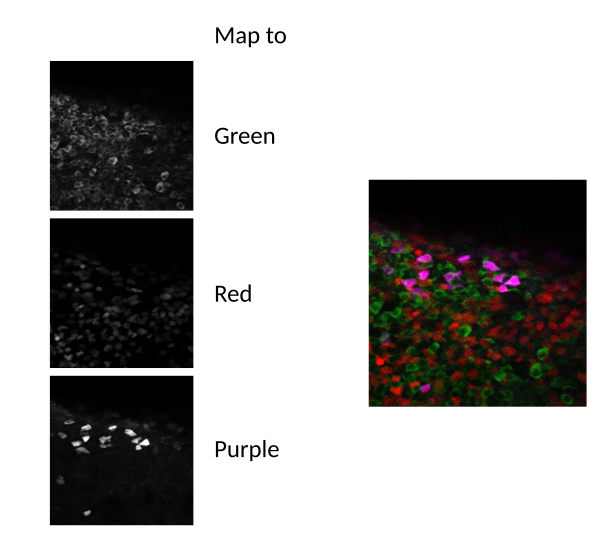
\includegraphics[height=180px]{pseudocolor.png}
    \end{figure}
\end{frame}

\begin{frame}
    {Look-up tables (LUTs)}
    Pseudocoloring is obtained through look-up tables (sometimes referred to as "palettes" or "colourmaps")

    \begin{figure}
        \centering
        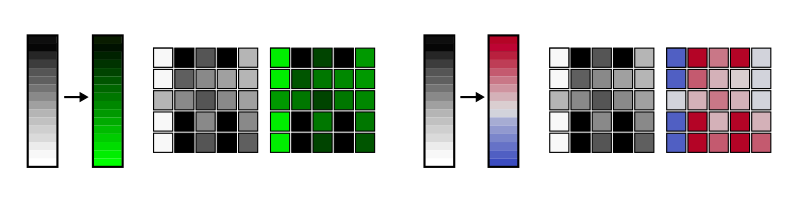
\includegraphics[width=400px]{lut.png}
        \caption{\centering Colourmaps can be sequential/linear or non sequential.

            Divergent and non-linear colour maps can be good to enhance differences in the image,

            but should be used with caution!}
    \end{figure}
\end{frame}

\begin{frame}
    {The Jet palette - when colourmaps go bad\dots}
    The Jet colourmap has for a long time been the standard palette in Matlab, is used in many pieces of software and is seen in many published articles. Jet is problematic because it can create artefacts in your data.

    \begin{figure}
        \centering
        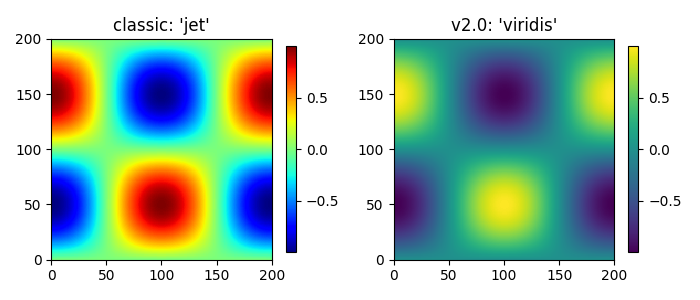
\includegraphics[width=300px]{jet_vs_viridis.png}

        \caption{\centering
            \color{gray}{Jet can create artefacts in the data. [Source: Matplotlib website]}
        }

        See also \url{https://www.youtube.com/watch?v=xAoljeRJ3lU}
        % \only<2>
        % {
        %     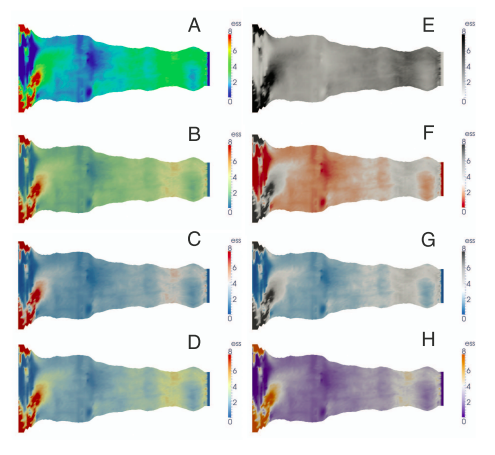
\includegraphics[width=170px]{borkin2011.png}
        %     \caption{\centering\color{gray}
        %         {\textit{Rainbow} palette resulted in significantly more diagnostic errors - Borkin 2011}}
        % }
    \end{figure}
\end{frame}

\begin{frame}
    {Colourmapping in Matplotlib}
    We can easily colourmap an image loaded in Matplotlib

    \only<1-2>{
        \begin{codebox}
            \texttt{import matplotlib.pyplot as plt\\
                img = imread("cells.tif")\\
                \# plt.subplots allows plotting more than one image\\
                \# side by side. It creates and returns a figure and\\
                \# a list of axes (the subplots)\\
                fig, ax = plt.subplots(ncols=3, nrows=1, figsize=(10, 6))\\
                \pause
                ax[0].imshow(img, cmap="gray")\\
                ax[1].imshow(img, cmap="viridis")\\
                ax[2].imshow(img, cmap="rainbow")\\
                plt.show()}
        \end{codebox}
    }
    \only<3>{
        \begin{figure}
            \centering
            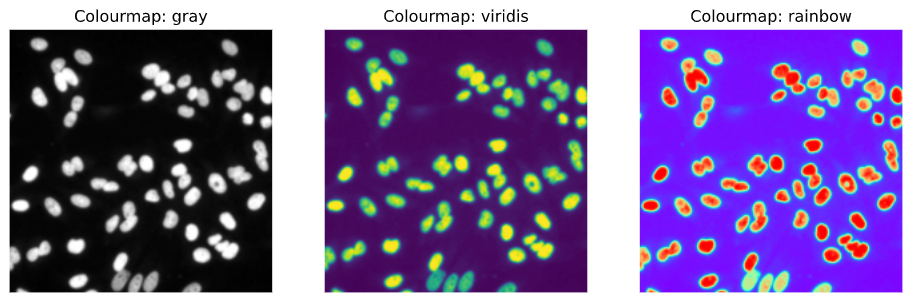
\includegraphics[width=\textwidth]{colourmaps.png}
            \caption{Check out the Matplotlib website for a list of colourmaps! \url{https://matplotlib.org/stable/tutorials/colors/colormaps.html}}
        \end{figure}
    }
\end{frame}

\begin{frame}
    {Image intensity vs visualized intensity}
    \texttt{imshow} has two parameters called \texttt{vmin} and \texttt{vmax} to control the \textbf intensity range of the image \textbf{on the screen}.

    For example, if you set \texttt{vmin=0} and \texttt{vmax=255}, then the image will be shown with 0 being black and 255 being white.
    If you set \texttt{vmax=100}, then any pixel with an intensity higher than 100 will be shown as white.
    \pause
    \begin{columns}
        \begin{column}{0.5\textwidth}
            \begin{codebox}
                \texttt{plt.imshow(img, vmin=0, vmax=255)\\
                    plt.imshow(img, vmin=0, vmax=50)\\
                    \# Automatically uses min and max of the image\\
                    plt.imshow(img)}
            \end{codebox}
        \end{column}
        \begin{column}{0.5\textwidth}
            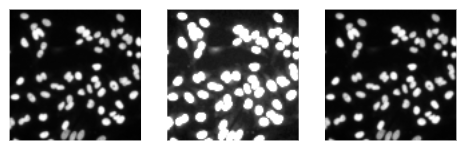
\includegraphics[width=\textwidth]{vmin_vmax.png}
        \end{column}
    \end{columns}

    IMPORTANT: the actual pixel intensity of these images are all the same we are just modifying how they are displayed on the screen.
\end{frame}

\begin{frame}
    {Practice time!}
    \centering
    \Large
    And now some practice on what we saw today!
\end{frame}

\end{document}

